
\chapter{Oscillazioni smorzate e forzate}


\section{Introduzione}
\subsection{Oggetto della ricerca}
L'oggetto di questa ricerca è lo studio delle oscillazioni smorzate e forzate di un pendolo. Studiando il variare delle oscillazioni con il variare della frequenza operativa della forzante, si studierà il fenomeno della risonanza.

\subsection{Strumenti}
\begin{center}
\begin{tabular}{l|l}
\midrule
Strumento & Precisione\\
\midrule
Calibro & $\pm 0.05$ mm\\ 
Sensore di rotazione & $\pm 0.00157$ rad\\ 
Alimentatore & $\pm 0.01$ V\\ 
\midrule 
\end{tabular}
\end{center}
L'attrezzatura utilizza è costituita da un disco metallico attaccato ad una puleggia. La puleggia è messa in oscillazione da un filo alle cui estremità vi sono un oscillatore  elettromeccanico e un sistema di due molle. Al disco è possibile avvicinare e allontanare un magnete, fissato su una vite. 

\subsection{Metodo in breve}
L'esperimento è suddiviso in tre fasi:

\begin{itemize}
\item \textbf{Oscillazioni pseudo-libere}
Si ponga in oscillazione il disco, con il magnete  posizionato lontano e l'oscillatore elettromeccanico spento. Si misuri il periodo delle oscillazioni libere.
\item \textbf{Oscillazioni smorzate}
Si avvicini il magnete al disco metallico. Il moto oscillatorio risulterà così smorzato per effetto delle correnti di Focault 
\item \textbf{Oscillazioni smorzate e forzate}
Per queste misurazioni, si metta in azione l'oscillatore elettromeccanico, che fornisce una componente forzante. Variando il voltaggio dell'alimentatore,  la frequenza di rotazione dell'oscillatore cambia. Si cerchi la frequenza di risonanza del sistema.
\end{itemize}

[se la consegnamo, aggiungi diagramma]

\section{Raccolta dati}

I seguenti grafici rappresentano la posizione in funzione del tempo delle oscillazioni in esame. Sono state rilevate da un sensore di moto rotatorio, collegato al disco metallico. 
Nella sezione "oscillazioni smorzate-forzate", ci siamo serviti di una fotocellula per misurare il periodo della forzante generata dall'oscillatore elettromeccanico. 

\subsection{Oscillazioni libere}

- Grafici posizione tempo 

\subsection{Oscillazioni smorzate}

- Grafici 
\subsection{Oscillazioni smorzate-forzate}

- Grafici

\section{Analisi dati}

\subsection{Oscillazioni libere}
In questa prima fase dell'analisi dei dati, estrapoliamo dalla posizione in funzione del tempo, il periodo dell'oscillazione libera. Essendo un sistema reale, risultata comunque smorzato dalla presenza di attriti. 


\subsection{Oscillazioni smorzate}

Abbiamo ricavato i valori dei parametri liberi utilizzando il programma DataStudio, e interpolando i dati con la seguente equazione:
$$ \theta (t) = A_0 e^{- \gamma t} \sin(wt+\phi)+\theta_0 $$


Dunque, noti $\omega$ e $\gamma$, è possibile calcolare $ \omega_0 $, cioè la pulsazione per le oscillazioni libere, tramite l'equazione:
$$ \omega = \sqrt{\omega_0^2 - \gamma^2} $$

e confrontarlo con il valore che avevamo ricavato interpolando direttamente il grafico delle oscillazioni libere

$$\omega_0 = 4.272\ rad/s$$

\subsubsection{4.80mm}

\begin{center}
\begin{tabular}{l|l|l}
\midrule
Parametri & Valore ricavato & $ \pm \sigma$ \\
\midrule
$A_0$ & 3.08 rad & 0.020\\
$\gamma$ & 0.197 $m^4/kg$& 0.0019\\
$\omega$ & -4.27 rad/s& 0.0019\\
$\phi$ & 1.93 rad & 0.0069 \\
$\theta_0$ & -1.53 rad& 0.0019 \\
\midrule
\end{tabular}
\end{center}

Il valore così calcolato è leggermente maggiore di quello ricavato dalla misurazione diretta. $$\omega_{0} = 4.275\ rad/s$$

Questo risultato è in perfetto accordo nei limiti della precisione dello strumento.
\subsubsection{2.80mm}

\begin{center}
\begin{tabular}{l|l|l}
\midrule
Parametri & Valore ricavato & $ \pm \sigma$ \\
\midrule
$A_0$ & 3.40 rad & 0.020\\
$\gamma$ & 0.636 $m^4/kg$& 0.0057\\
$\omega$ & -4.25 $rad/s$& 0.0064\\
$\phi$ & 2.38 $rad$ & 0.0076 \\
$\theta_0$ & -0.57 $rad$& 0.0038 \\
\midrule
\end{tabular}
\end{center}

$$\omega_{0} = 4.297\ rad/s$$

\subsubsection{1.00mm}

\begin{center}
\begin{tabular}{l|l|l}
\midrule
Parametri & Valore ricavato & $ \pm \sigma$ \\
\midrule
$A_0$ & 18600 rad & 1300 \\
$\gamma$ & 1.50 $m^4/kg$& 0.0011\\
$\omega$ & 4.02 rad/s& 0.0077\\
$\phi$ & 26.3 rad & 0.0046 \\
$\theta_0$ & 0.055 rad& 0.0016 \\
\midrule
\end{tabular}
\end{center}

$$\omega_{0} = 4.291\ rad/s $$

\subsection{Oscillazioni smorzate-forzate}
Tramite l'interpolazione dei grafici di posizione angolare in funzione del tempo con una funzione\\
sinosuidale, sono stati trovati i valori dell'ampiezza e del periodo di ognuna delle oscillazioni.

Dopodiché abbiamo interpolato questi dati con il programma DataStudio, secondo la funzione
$$ A(\omega) = \frac{M_0}{\sqrt{ ({\omega_0}^2-\omega^2)^2 + 4\gamma^2\omega^2}} $$

e lasciando liberi i parametri $M_0$, $\gamma$ e $\omega_0$ abbiamo trovato alcuni valori. Abbiamo omesso di trascrivere gli errori quando questi erano palesemente trascurabili.

\clearpage

\subsubsection{4.80mm}
\begin{center}

\includegraphics[scale=0.75]{"../grafici/Magnetea48mm"}
\end{center}
\begin{center}
\begin{tabular}{l|l|l}
$\omega$ (rad/s) & Periodo (s) & A (rad) \\
\midrule
1.15	& 5.45 & 0.89\\
1.31	& 4.78 & 0.94\\
1.75	& 3.57 & 1.05\\
1.97	& 3.19 & 1.09\\
2.42	& 2.59 & 1.30\\
2.55	& 2.46 & 1.30\\
3.05    & 2.06 & 1.84\\
3.31	& 1.90 & 1.91\\
3.69	& 1.70 & 3.42\\
3.95	& 1.59 & 6.35\\
4.94	& 1.27 & 2.48\\
5.19	& 1.21 & 1.74\\
5.51	& 1.14 & 1.19 \\
\midrule

\end{tabular}
$$ \omega_0 = 4.25\ rad/s $$
$$ \gamma = 0.193\ s^{-1}$$
$$ M_0 = 15.3\ s$$


\end{center}




\subsubsection{2.80mm}
\begin{center}
\begin{tabular}{l|l|l}
$\omega$ (rad/s) & Periodo (s) & A (rad) \\
\midrule
3.14 & 2.00 & 1.68 \\
3.85 & 1.63 & 2.95 \\
4.36 & 1.44 & 3.22 \\
4.83 & 1.30 & 2.17 \\
5.06 & 1.24 & 1.67 \\
5.46 & 1.15 & 1.20 \\
5.71 & 1.10 & 0.99 \\
6.40 & 0.98 & 0.68 \\
7.06 & 0.89 & 0.51 \\
8.49 & 0.74 & 0.26 \\
\midrule
\end{tabular}
\end{center}
\includegraphics[scale=0.75]{"../grafici/Magnetea28mm"}



$$ \omega_0 = 4.26\ rad/s $$
$$ \gamma = 0.543\ s^{-1} $$
$$ M_0 = 15.6\ s$$


\subsubsection{1.00mm}
\begin{center}
\begin{tabular}{l|l|l}
$\omega$ (rad/s) & Periodo (s) & A (rad) \\
\midrule
3.12 & 2.01 & 1.33 \\
3.39 & 1.85 & 1.42 \\
3.76 & 1.67 & 1.45 \\
4.07 & 1.54 & 1.47 \\
4.52 & 1.39 & 1.31 \\
4.79 & 1.31 & 1.18 \\
5.15 & 1.22 & 1.01 \\
5.28 & 1.19 & 0.88 \\
5.76 & 1.09 & 0.76 \\
6.10 & 1.03 & 0.65 \\
6.75 & 0.93 & 0.49 \\
7.39 & 0.85 & 0.39 \\
\midrule
\end{tabular}
\end{center}
\includegraphics[scale=0.75]{"../grafici/Magnetea10mm"}


$$ \omega_0 = 4.37\ rad/s $$
$$ \gamma = 1.40 \pm 0.14\ s^{-1}$$
$$ M_0 = 17.1 \pm 1.4\ s$$

Spiegazione fenomeno risonanza

% 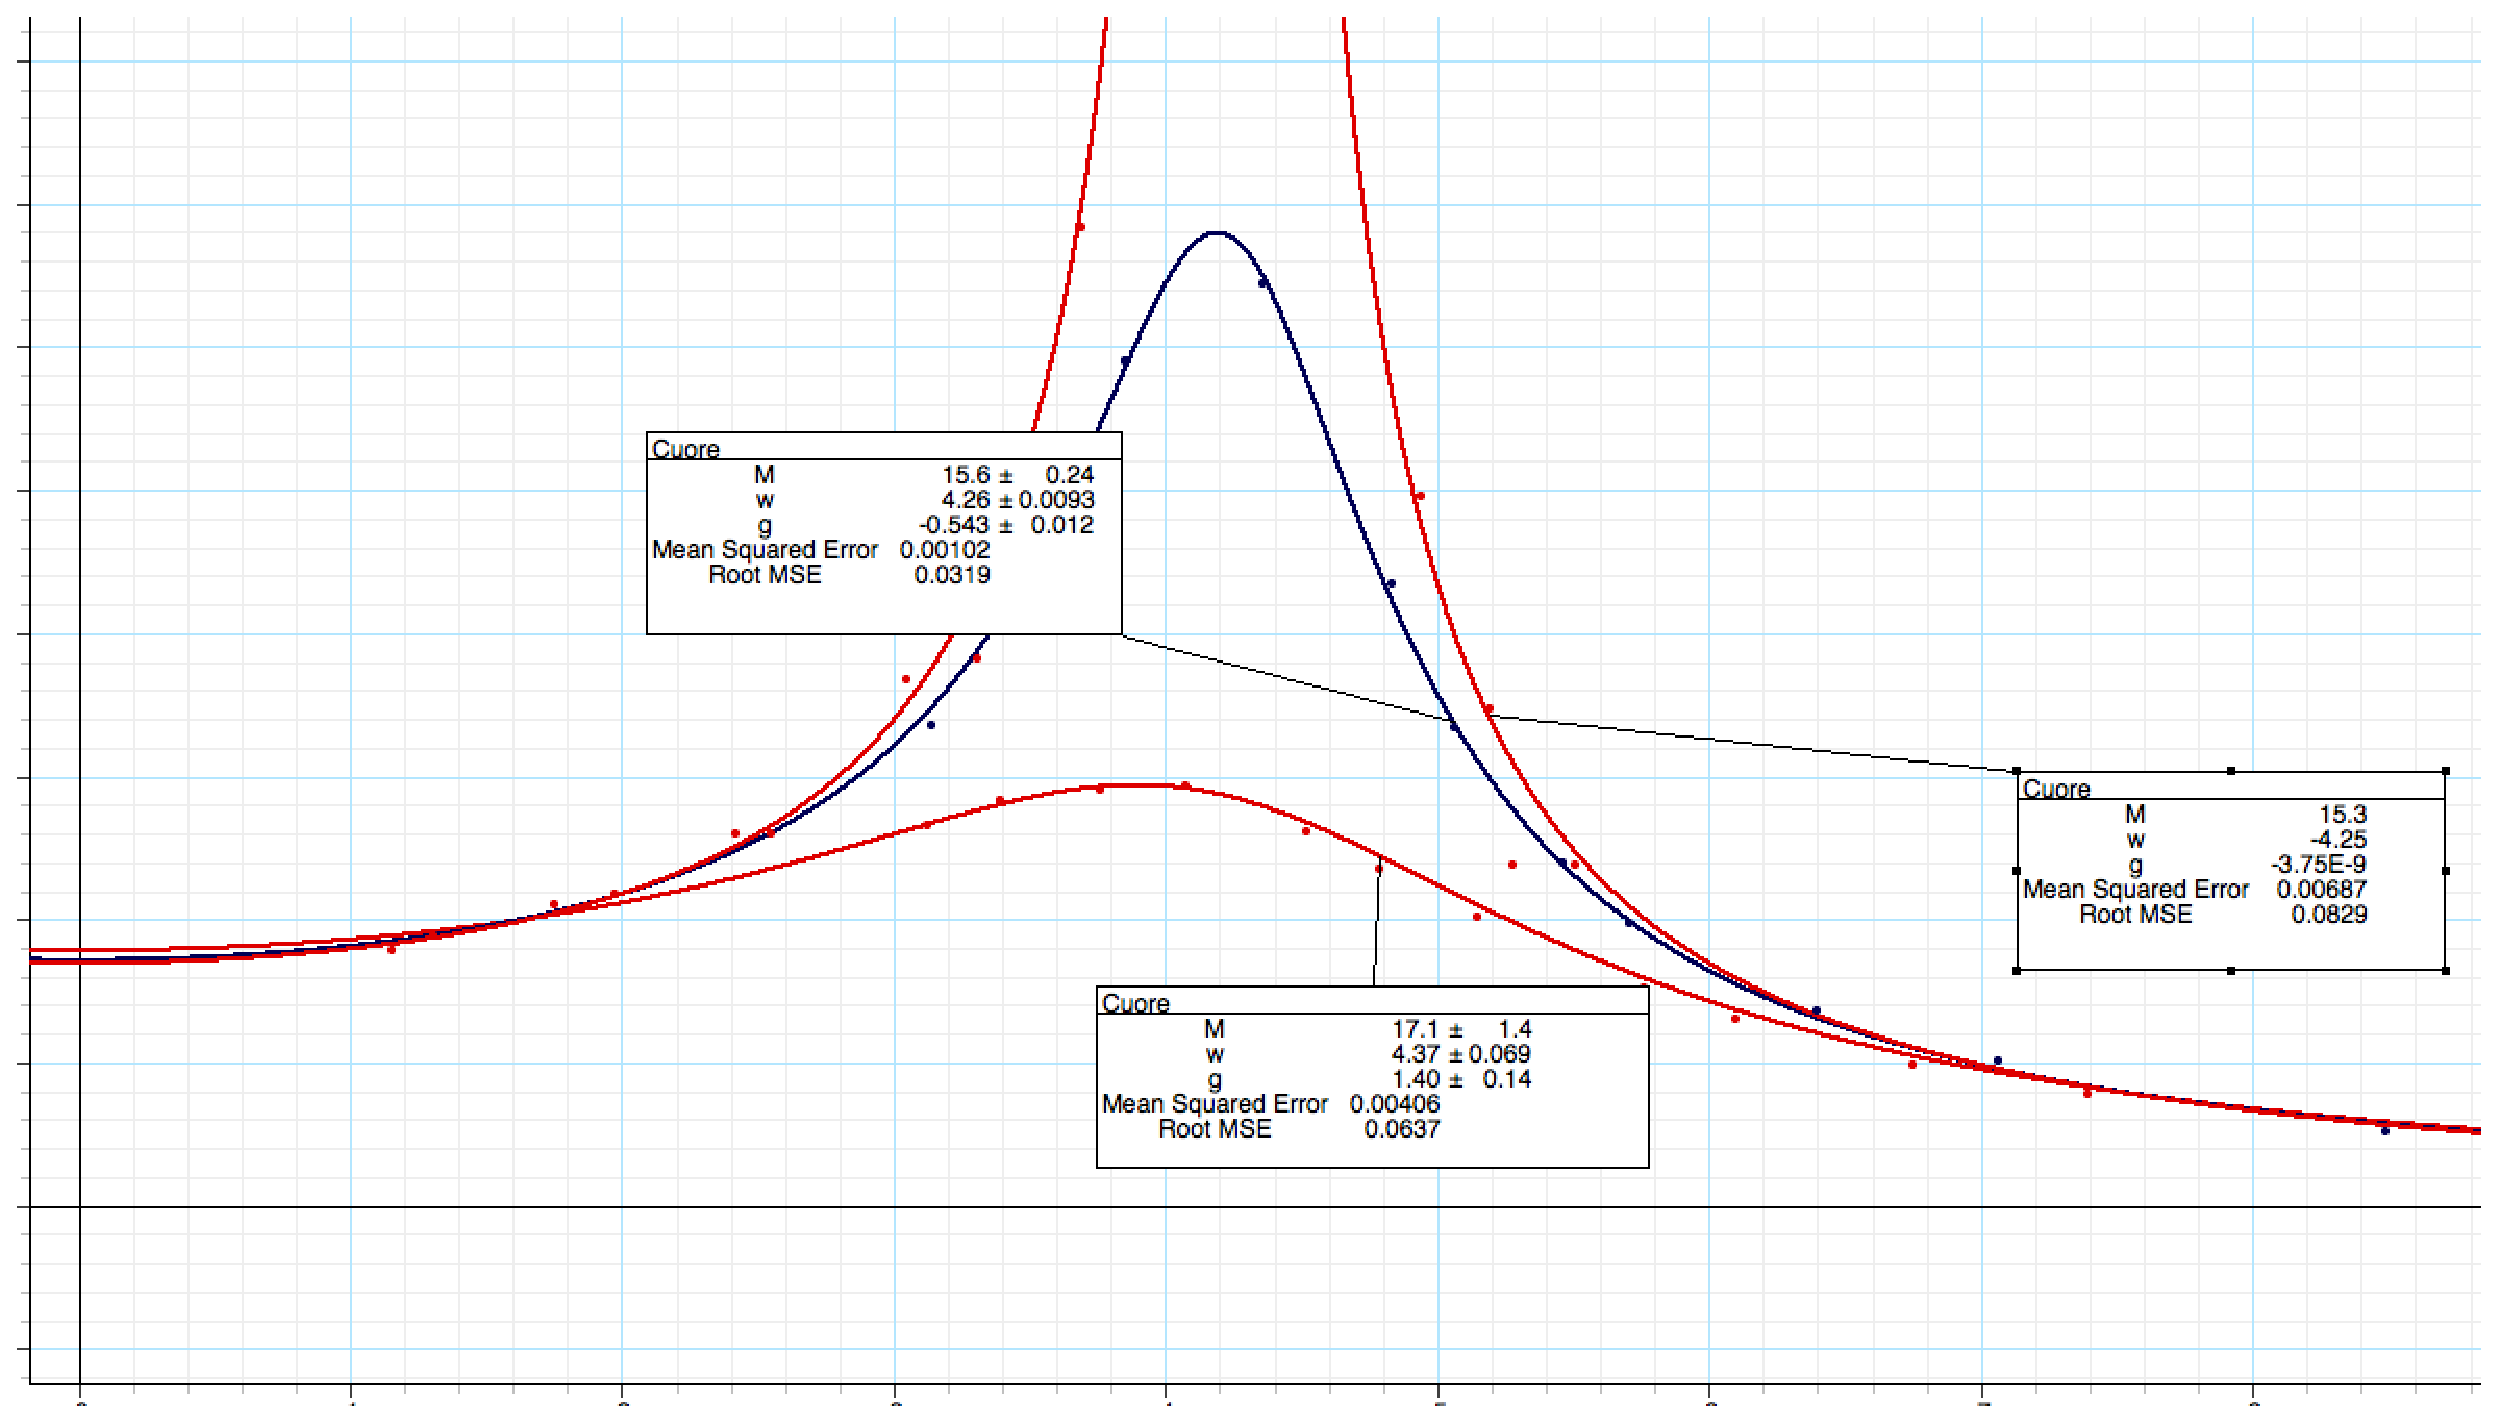
\includegraphics[scale=0.2]{graf}
%Fare grafico tutti insieme?

\section{Conclusioni}
L'esperimento è riuscito un sacco.

